\subsection{Экономическая эффективность}

\begin{table}[b]
    \centering
    \caption{Стоимость комплектующих сервера}
    \label{tab:server_price}
    \begin{tabu}to \linewidth{XX[1,c,m]X[1,r,m]}
        \toprule
        Компонент & Название & Стоимость, руб \\
        \midrule
        Процессор          & AMD Ryzen 5 2600                          & 8 980  \\
        Материнская плата  & Asus PRIME X370-PRO                       & 12 590 \\
        Оперативная память & Patriot Signature 16GB PSD416G26662, 2 шт & 9 998   \\
        Видеокарта         & Sapphire Radeon RX 580 PULSE 8GB          & 16 138  \\
        Накопитель         & Samsung 860 EVO 500 ГБ                    & 6 060  \\
        Блок питания       & Be quiet! Straight Power 11 850 Вт        & 14 503 \\
        \midrule
        Итог & & 68 269 \\
        \bottomrule
    \end{tabu}
\end{table}

\begin{table}[t]
    \centering
    \caption{Стоимость комплектующих рабочего ПК}
    \label{tab:pc_price}
    \begin{tabu}to \linewidth{XX[1,c,m]X[1,r,m]}
        \toprule
        Компонент & Название & Стоимость, руб \\
        \midrule
        Процессор          & Intel Core i3-9100F                 & 5 721 \\
        Материнская плата  & Asus PRIME B360M-A                  & 5 893 \\
        Оперативная память & Crucial Value DDR4 4Gb CT4G4DFS824A & 1 331 \\
        Видеокарта         & Интегрированная в процессор         & —     \\
        Накопитель         & Kingston A400 120 ГБ                & 1 960  \\
        Блок питания       & FSP ATX-500PNR                      & 2 366  \\
        \midrule
        Итог & & 17 271 \\
        \bottomrule
    \end{tabu}
\end{table}

Для оценки экономической эффективности нужно сравнить затраты на аппаратное и
программное обеспечение, используемое в проекте. Цены на компьютерные комплектующие
взяты с сервиса агрегации цен E-katalog \cite{ref:eeekatalog}. Цены на ПО взяты с сайтов
официальных дистрибуторов ПО (или их представителей в Российской Федерации).  Для
отсутствующих в продаже компонентов взяты их современные аналоги, сравнимые по
производительности.

Т.к. сервер для демонстрации возможностей данного проекта собран из обычных
потребительских комплектующих, в таблице указана их стоимость. Стоит отметить, что для
сборки полноценного сервера стоит использовать специализированные серверные 
комплектующие. Их стоимость выше, однако и производительность при этом отличается в
большую сторону, что может быть полезно для дальнейшего увеличения производительности и
надежности всей системы.

Стоимость серверных комплектующих приведена в таблице \ref{tab:server_price},
комплектующих ПК — в таблице \ref{tab:pc_price}. В расчетах не учитывается стоимость
корпуса. С учетом стоимости Raspberry Pi 3 Model B, корпуса и блока питания в
6000~рублей при покупке от 5~шт. \cite{ref:raspberry_price} построены графики
зависимости стоимости от количества клиентов (см. рисунок~\ref{pic:hw_price_chart}).

\begin{figure}[h]
    \center
    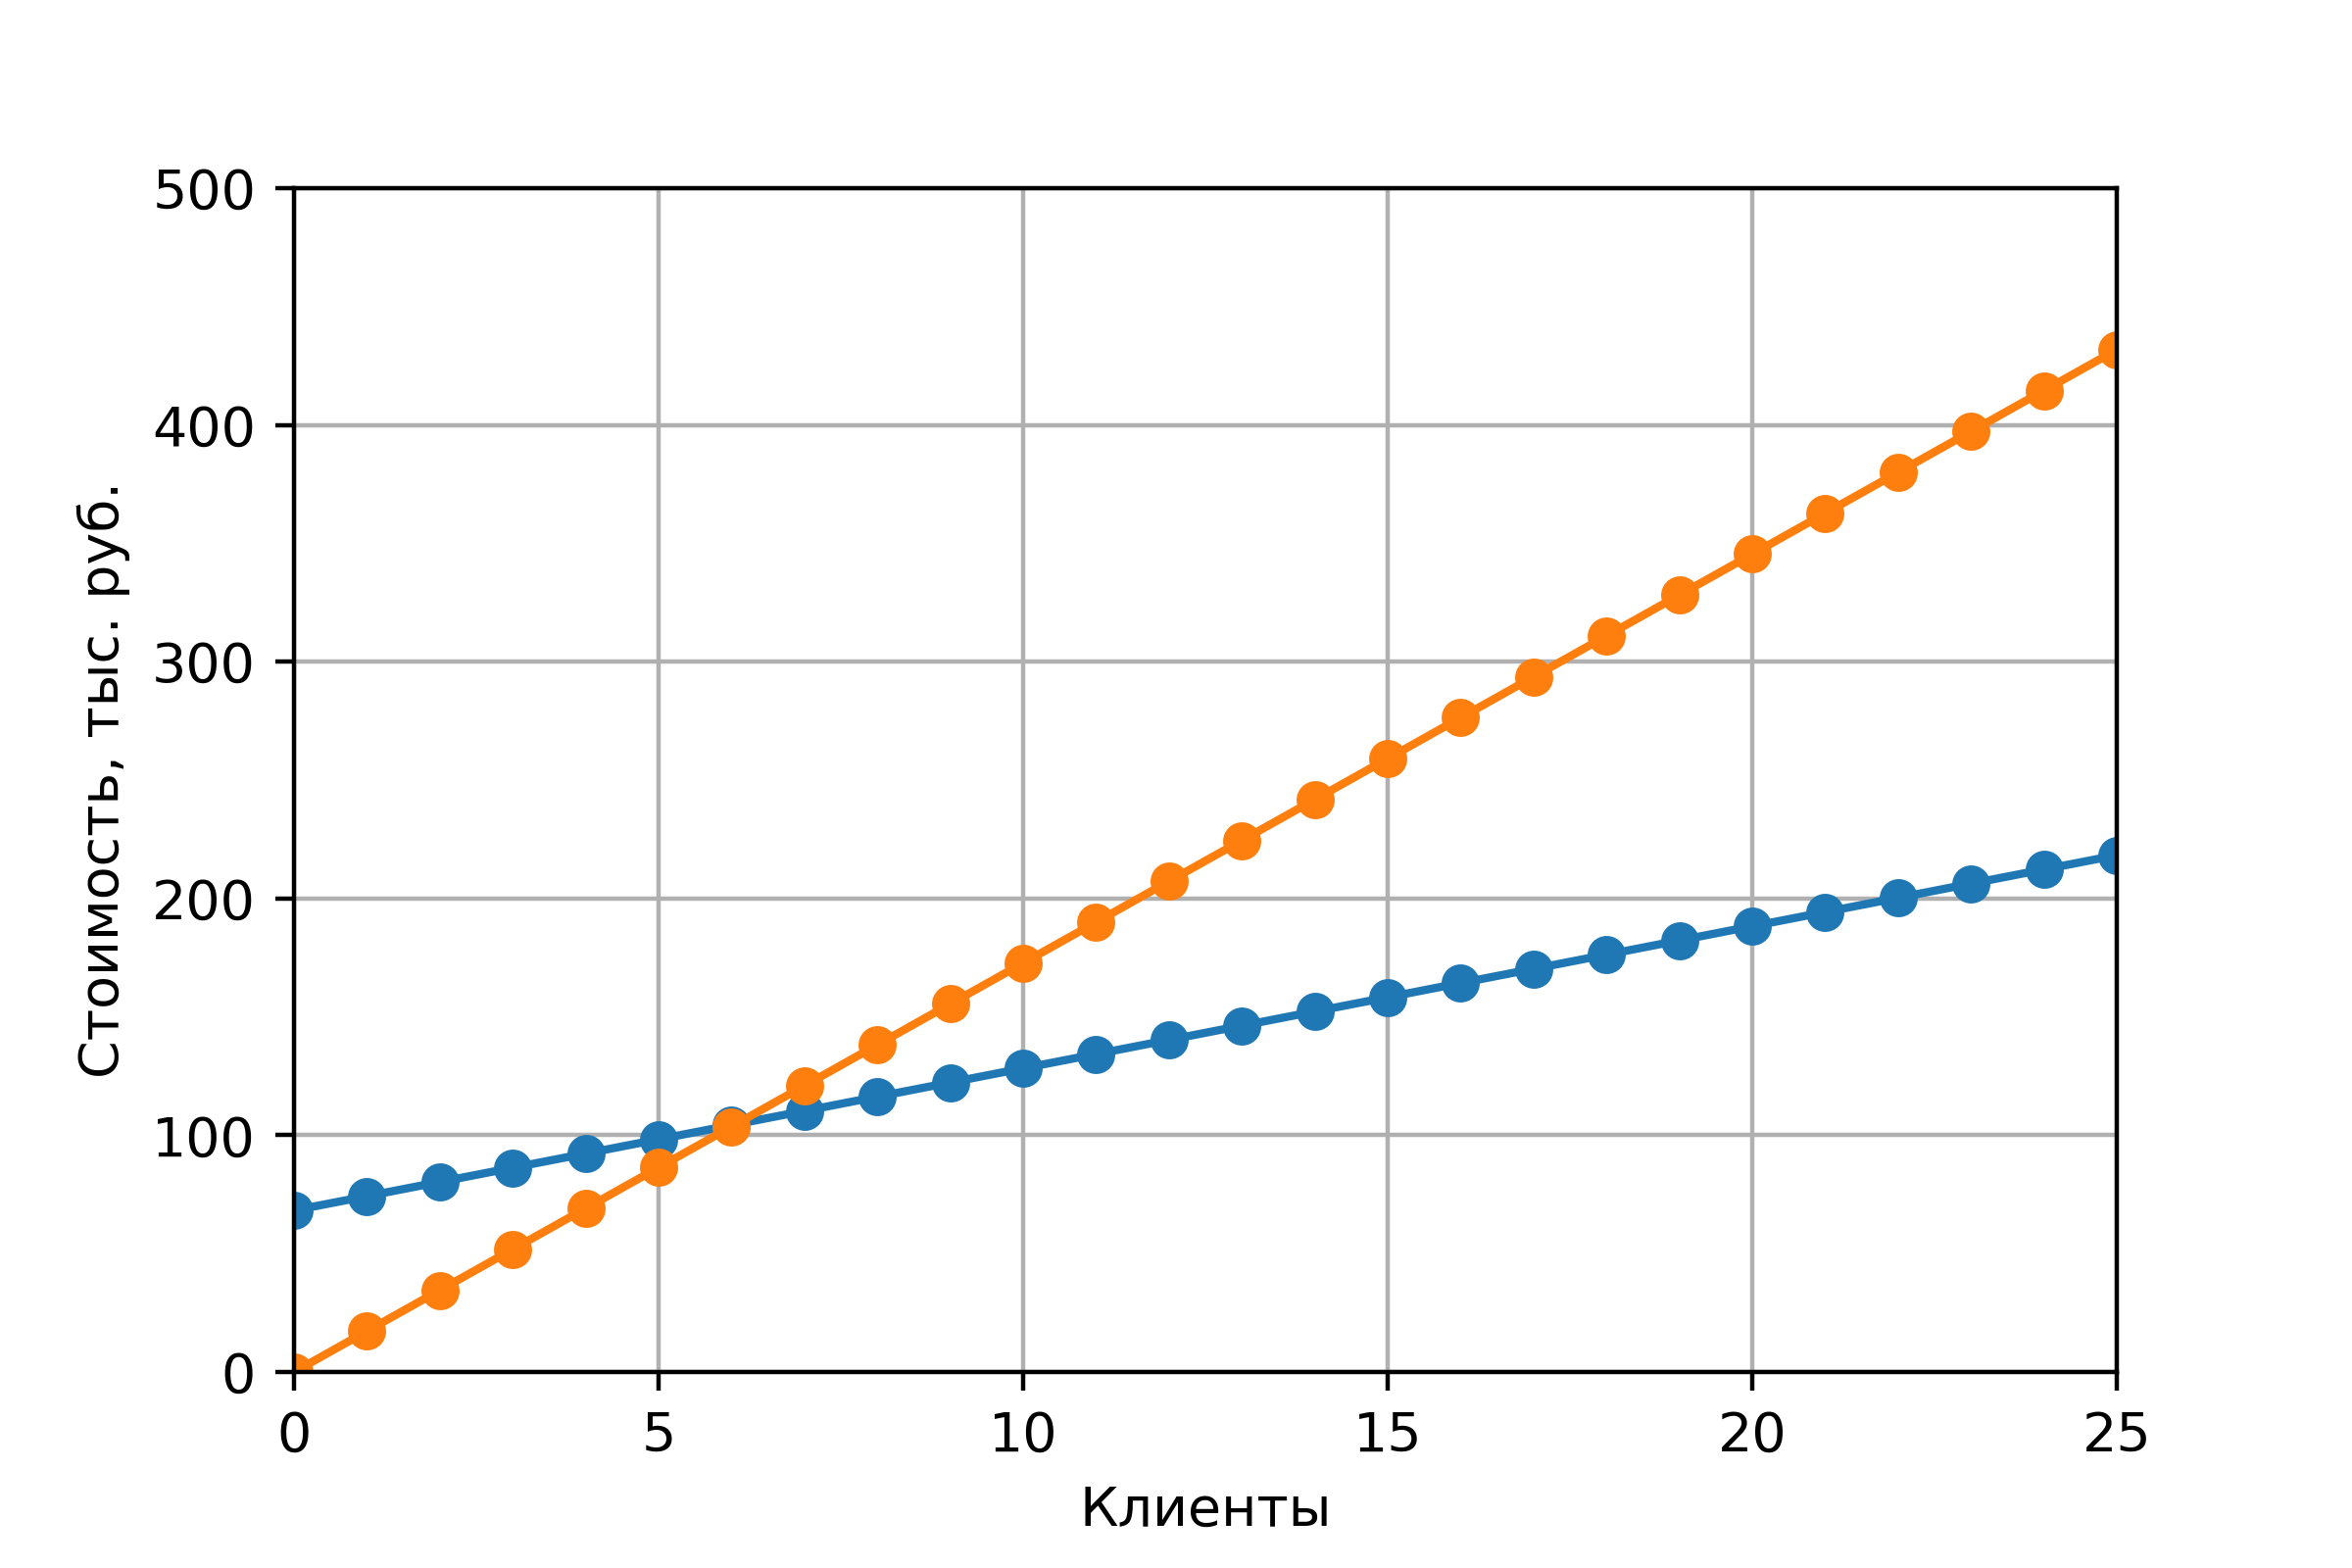
\includegraphics[width=\linewidth]{hw_price_chart}
    \caption{Зависимость стоимости системы от количества клиентов}
    \label{pic:hw_price_chart}
\end{figure}

Тут табличка с лицензиями виндовс

Тут табличка с лицензиями солида

Таким образом, можно сделать вывод о экономической целесообразности реализации данного
проекта. По сравнению с используемой на кафедре системой из полноценных компьютеров
(толстых клиентов), система тонких клиентов дает возможность значительно снизить затраты
при подключении требуемого количества клиентов, получая более высокую производительность
рабочих мест.
При подключении 25 клиентов, что является максимально возможным количеством
пользователей для используемой лицензии Windows Server Essentials, экономия средств на
программное обеспечение, составляет XX\%, на аппаратное — XX\%. Стоит отметить, что при
необходимости дальнейшей модернизации, достаточно будет обновить аппаратное обеспечение
только серверной части, что также уменьшает затраты на оборудование.
